\chapter{Approach}\label{chap:approach}
\section{Extract data}    
There are multiple repositories of Galaxy tools stored at GitHub \footnote{One example:\url{https://github.com/galaxyproject/tools-iuc/tree/master/tools}}. In each of the tool repository, there are $xml$ files starting with a $<tool>$ tag. We read all of these $xml$ files, extract information from a few of the attributes and collect them in a $tabular$ file.
    
\subsection{Select tools attributes}
A tool has multiple attributes like input and output file types, help text, name, description, citations and some more. But all of these attributes are not important and do not generally identify a tool exclusively. We consider some of these attributes:
\begin{itemize}
	\item Input and output file types
	\item Name and description
	\item Help text
\end{itemize}
Moreover, we combine the input and output file types and name and description respectively as they are of similar nature. These two combined attributes give complete information about a tool file types and its functionality. We also consider help text attribute which is larger in size compared to the previous two. At the same time, they are empty for few tools. Apart from being large in size, this attribute is noisy as well. It provides more information about the usage of a tool. Generally, in the first few lines, it gives a detailed explanation of the tool functions. Further, it explains how the input data should be supplied to a tool or how an input data looks like. Hence, much of the information present in this attribute is not important. Because of noise present in this attribute, we decide to use only upto first $4$ lines which illustrates the core functionality of the tool. The decision to select only first $4$ lines is empirical. The rest of the information in help text is discarded. 

\subsection{Clean data}
\subsubsection{Remove duplicates and stopwords}
    The collected data for tools is raw containing lots of commonplace and duplicate items which do not add value. These items should be removed to get $tokens$ which are unique and useful. For example, a tool $bamleftalign$ has input files as $bam, fasta$ and output file as $bam$. While combining the file types, we discard the repeated file types and in this case, we consider file types as $bam, fasta$. The other attributes we deal with are different from the file types. The files types are discrete items but in attributes like name and description and help text, the account is in a human language. The explanation contains complete or partially complete sentences in $English$. Hence, to process this information, we need startegies that are prevalent in natural language processing \footnote{\url{https://www.ncbi.nlm.nih.gov/pmc/articles/PMC3168328/}}. The sentences we write in $English$ contain many words and has different parts. These parts include subject, object, preposition, interjection, verbs, adjectives, adverbs, articles and many others. For our processing, we need only those tokens (words) which categorize a tool uniquely and do away with multiple parts of speech present in the statements. For example, a tool named $tophat$ has name and description as "TopHat for Illumina Find splice junctions using RNA-seq data". The words like $for$, $using$ and $data$ do not give much value as they must be present for many tools. These words are called as "stop words" \footnote{\url{https://www.ranks.nl/stopwords}} and we selectively discard them. In addition, we remove numbers and convert all the tokens to lower case.
   
\subsubsection{Use stemming}
After removing duplicates and stop words, our data is clean and contain tokens which uniquely identify corresponding tools. When we frame sentences, we follow grammar which constrains us to use different forms of the same word in varying contexts. For example, a word $regress$ can be used in multiple forms as $regresses$ or $regression$ or $regressed$. They share the same root and point towards the same concept. If many tools use this word in varying forms, it is beneficial to converge all the different forms of a word to one basic form. This is called stemming \footnote{\url{https://nlp.stanford.edu/IR-book/html/htmledition/stemming-and-lemmatization-1.html}}. We use nltk \footnote{\url{http://www.nltk.org/}} package for stemming.

\begin{figure}[h]
\begin{centering}
    {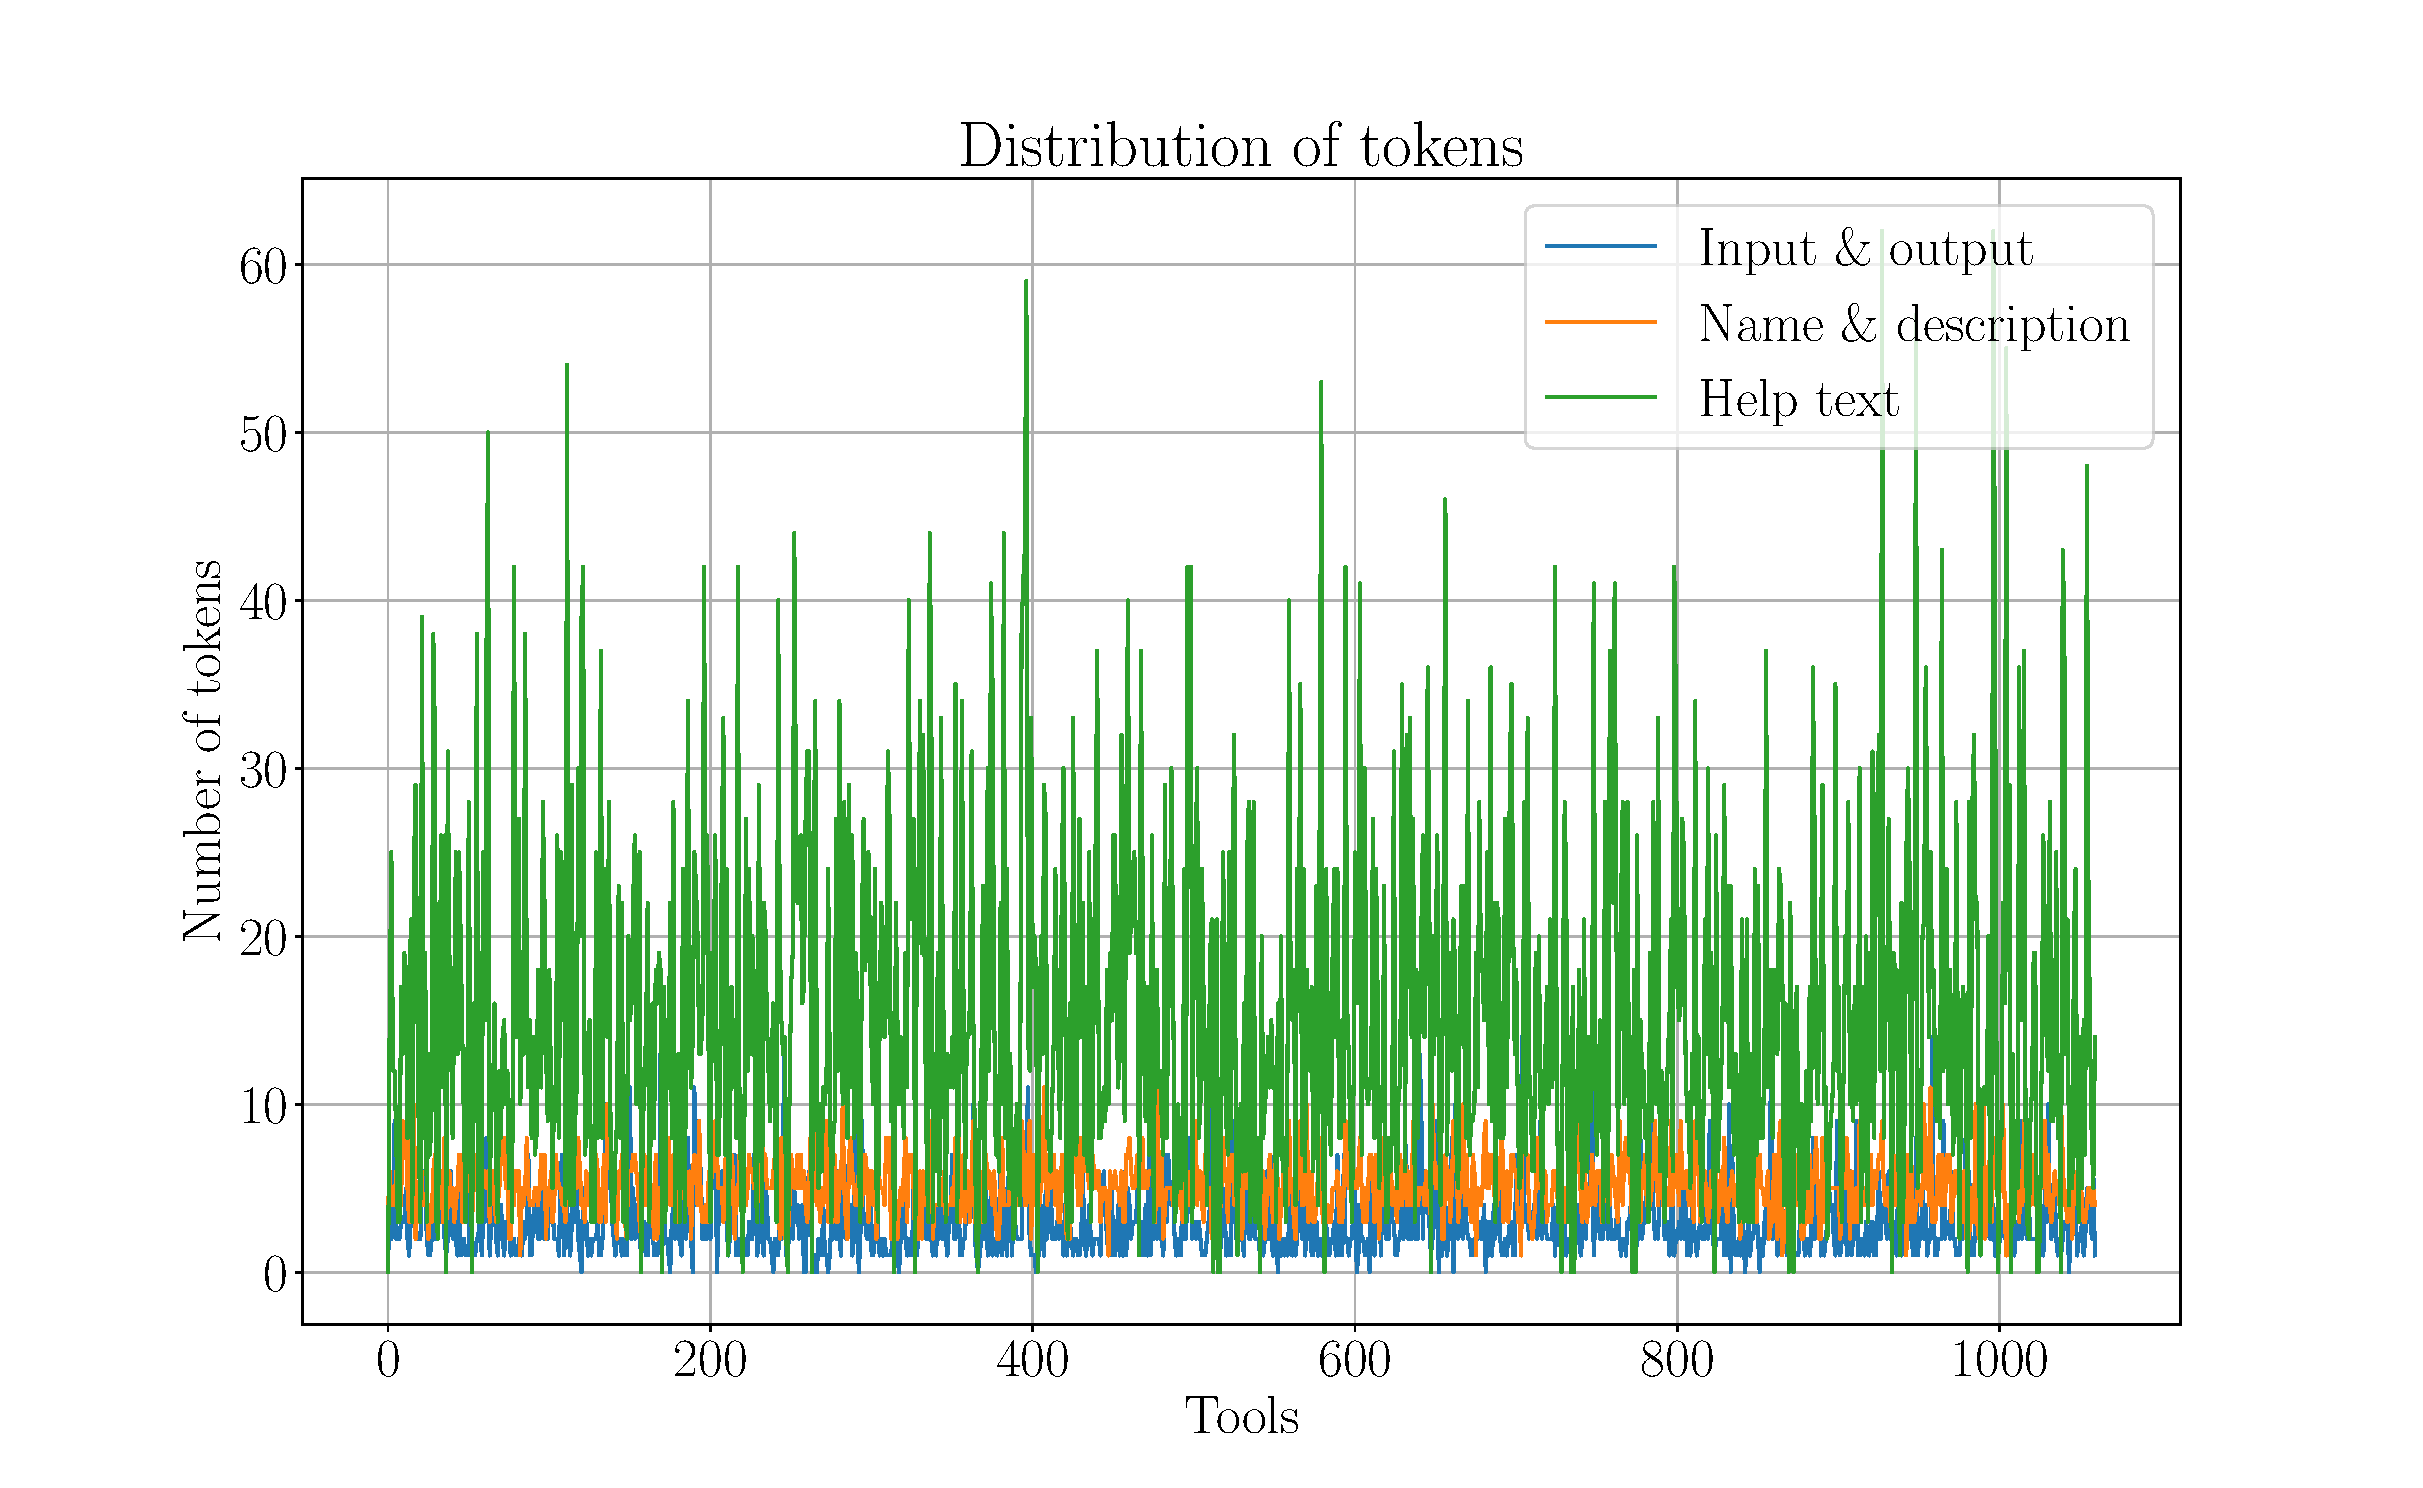
\includegraphics[scale=0.33]{figures/Tokens_dist.pdf}}
    \caption[Tokens distribution]{\textbf{Distribution of tokens}: the plot shows the distribution of tokens for all the attributes. The help text has the most number of tokens for all tools and input and output has the least number of tokens.}
\end{centering}
\end{figure}

\subsubsection{Refine tokens}
    At this stage of tools preprocessing, we have a set of good tokens for each attribute whic are input and output file types, name and description and help text. Let's call these sets as $documents$. The tokens present in these documents do not carry equal importance. Some tokens are more relevant to the document and some not so relevant . We need to find out importance factor for all tokens in a document. Using these factors, we can arrange them in big, sparse documents-tokens matrix. In this matrix, each row represents a document and each column belongs to one token. To compute these relevance scores, we use bestmatch25. Let's associate some variables to be used in explaining this algorithm.
    \begin{itemize}
	\item Token frequency \footnote{\url{https://nlp.stanford.edu/IR-book/pdf/06vect.pdf}} $tf$
	\item Inverted document frequency $idf$
	\item Average document length $|D|_{avg}$
	\item Number of documents $N$
	\item Size of a document $|D|$
\end{itemize}
    
First of all, token frequency ($tf$) specifies the count of a token's occurrence in a document. If a token $regress$ appears twice in a document, its $tf$ is $2$. This can also be understood as a weight given to this term. Inverted document frequency for a token is defined as:

\begin{equation}
idf = \log \frac{N}{df}
\end{equation}
 
where $df$ is the count of the documents in which this token is present and $N$ is the total number of documents. If we randomly sample a document, then the probability of this token to be present in this document is $ p_i = \frac{df}{N} $. From information theory, we can say that the information contained by this event is $ - \log p_i $. The entity $idf$ is higher when a token appears less number of documents which means that this token is a good candidate for representing the document and possesses higher power to distinguish between documents. The tokens which appear in many documents are not good representatives. Average document length is the average number tokens for all the documents. Size of a document is the count of all the tokens for that document \cite{Robertson:2009:PRF:1704809.1704810}. 


\begin{equation}
\alpha = (1-b) + \frac{b \cdot |D|}{|D|_{avg}}
\end{equation}

\begin{equation}
tf^* = tf \cdot \frac{k+1}{k \cdot \alpha + tf}
\end{equation}

\begin{equation}
BM25_{score} =tf^* \cdot idf
\end{equation}

where $k$ and $b$ are hyperparameters. Using the equation $4$, we compute the relevance score for each token in all the documents. Table 1 shows some sample scores for a few documents where the tokens are present with their respective relevance scores. In this way, we arrange document-tokens matrix for all the attributes of tools. For input and output file types, these matrix entries will have only two value, $1$ if a token is present for a document and $0$ if not. For other attributes, relevance scores are positive real numbers. This strategy of representing documents with their tokens is called vector space model as each document represents a vector of tokens.

\begin{table}[ht]
\begin{center}
    \begin{tabular}{|l|l|l|l|l|l|}
        \hline
        Documents/tokens   & regress & linear & gap & mapper & perform \\ \hline
        LinearRegression   & 5.22 & 4.1 & 0.0 & 0.0  & 3.84 \\ \hline
        LogisticRegression & 3.54 & 0.0 & 0.0 & 0.0  & 2.61 \\ \hline
        Tophat2            & 0.0  & 0.0 & 1.2 & 1.47 & 0.0 \\ \hline
        Hisat              & 0.0  & 0.0 & 0.0 & 0.0  & 0.0 \\ \hline
    \end{tabular}
    \end{center}
    \caption[Documents-tokens matrix]{\textbf{Document-tokens matrix}: it stores relevance scores for each token for all the documents\\}
    \label{tab:accuracy}
\end{table}

Figure 4 shows the heatmaps for documents-tokens matrices that belong to input and output file types and name and description. We can see that these plots are sparse. Each entry in these matrices contain BM25 score for each token in every document. The representation shows how to find tokens which are good representatives of documents with a weighted by their relevance factors. But, they do not tell un anything about the co-occurence of a few tokens in a document. It tells us that a token is important for a document if the BM25 score is higher but it does not tell us anything about its relation to other tokens. Due to this shortcoming, it does not acknowledge the presence of "concepts" or "context" hidden in a document. A concept in document can be realised when we see the relation among a few words. To illustrate this idea, let's take an example of three words - "New York City". These three words mean little or point to different things if looked at separately. But, if we see them together, it points towards a concept. This vector space model lacks the ability to find the correlation among tokens. To enable the vector space model to learn this hidden concepts and find correlation among multiple tokens, we explore two ideas
\begin{itemize}
\item Latent Semantic Indexing/Analysis \footnote{\url{http://lsa.colorado.edu/papers/dp1.LSAintro.pdf}}
\item Paragraph Vectors
\end{itemize}

Using these approaches, we learn dense, $n$ dimensional vector for each document instead of using sparse vectors as shown in figure 5. 

\begin{figure}[h]
\begin{centering}
    {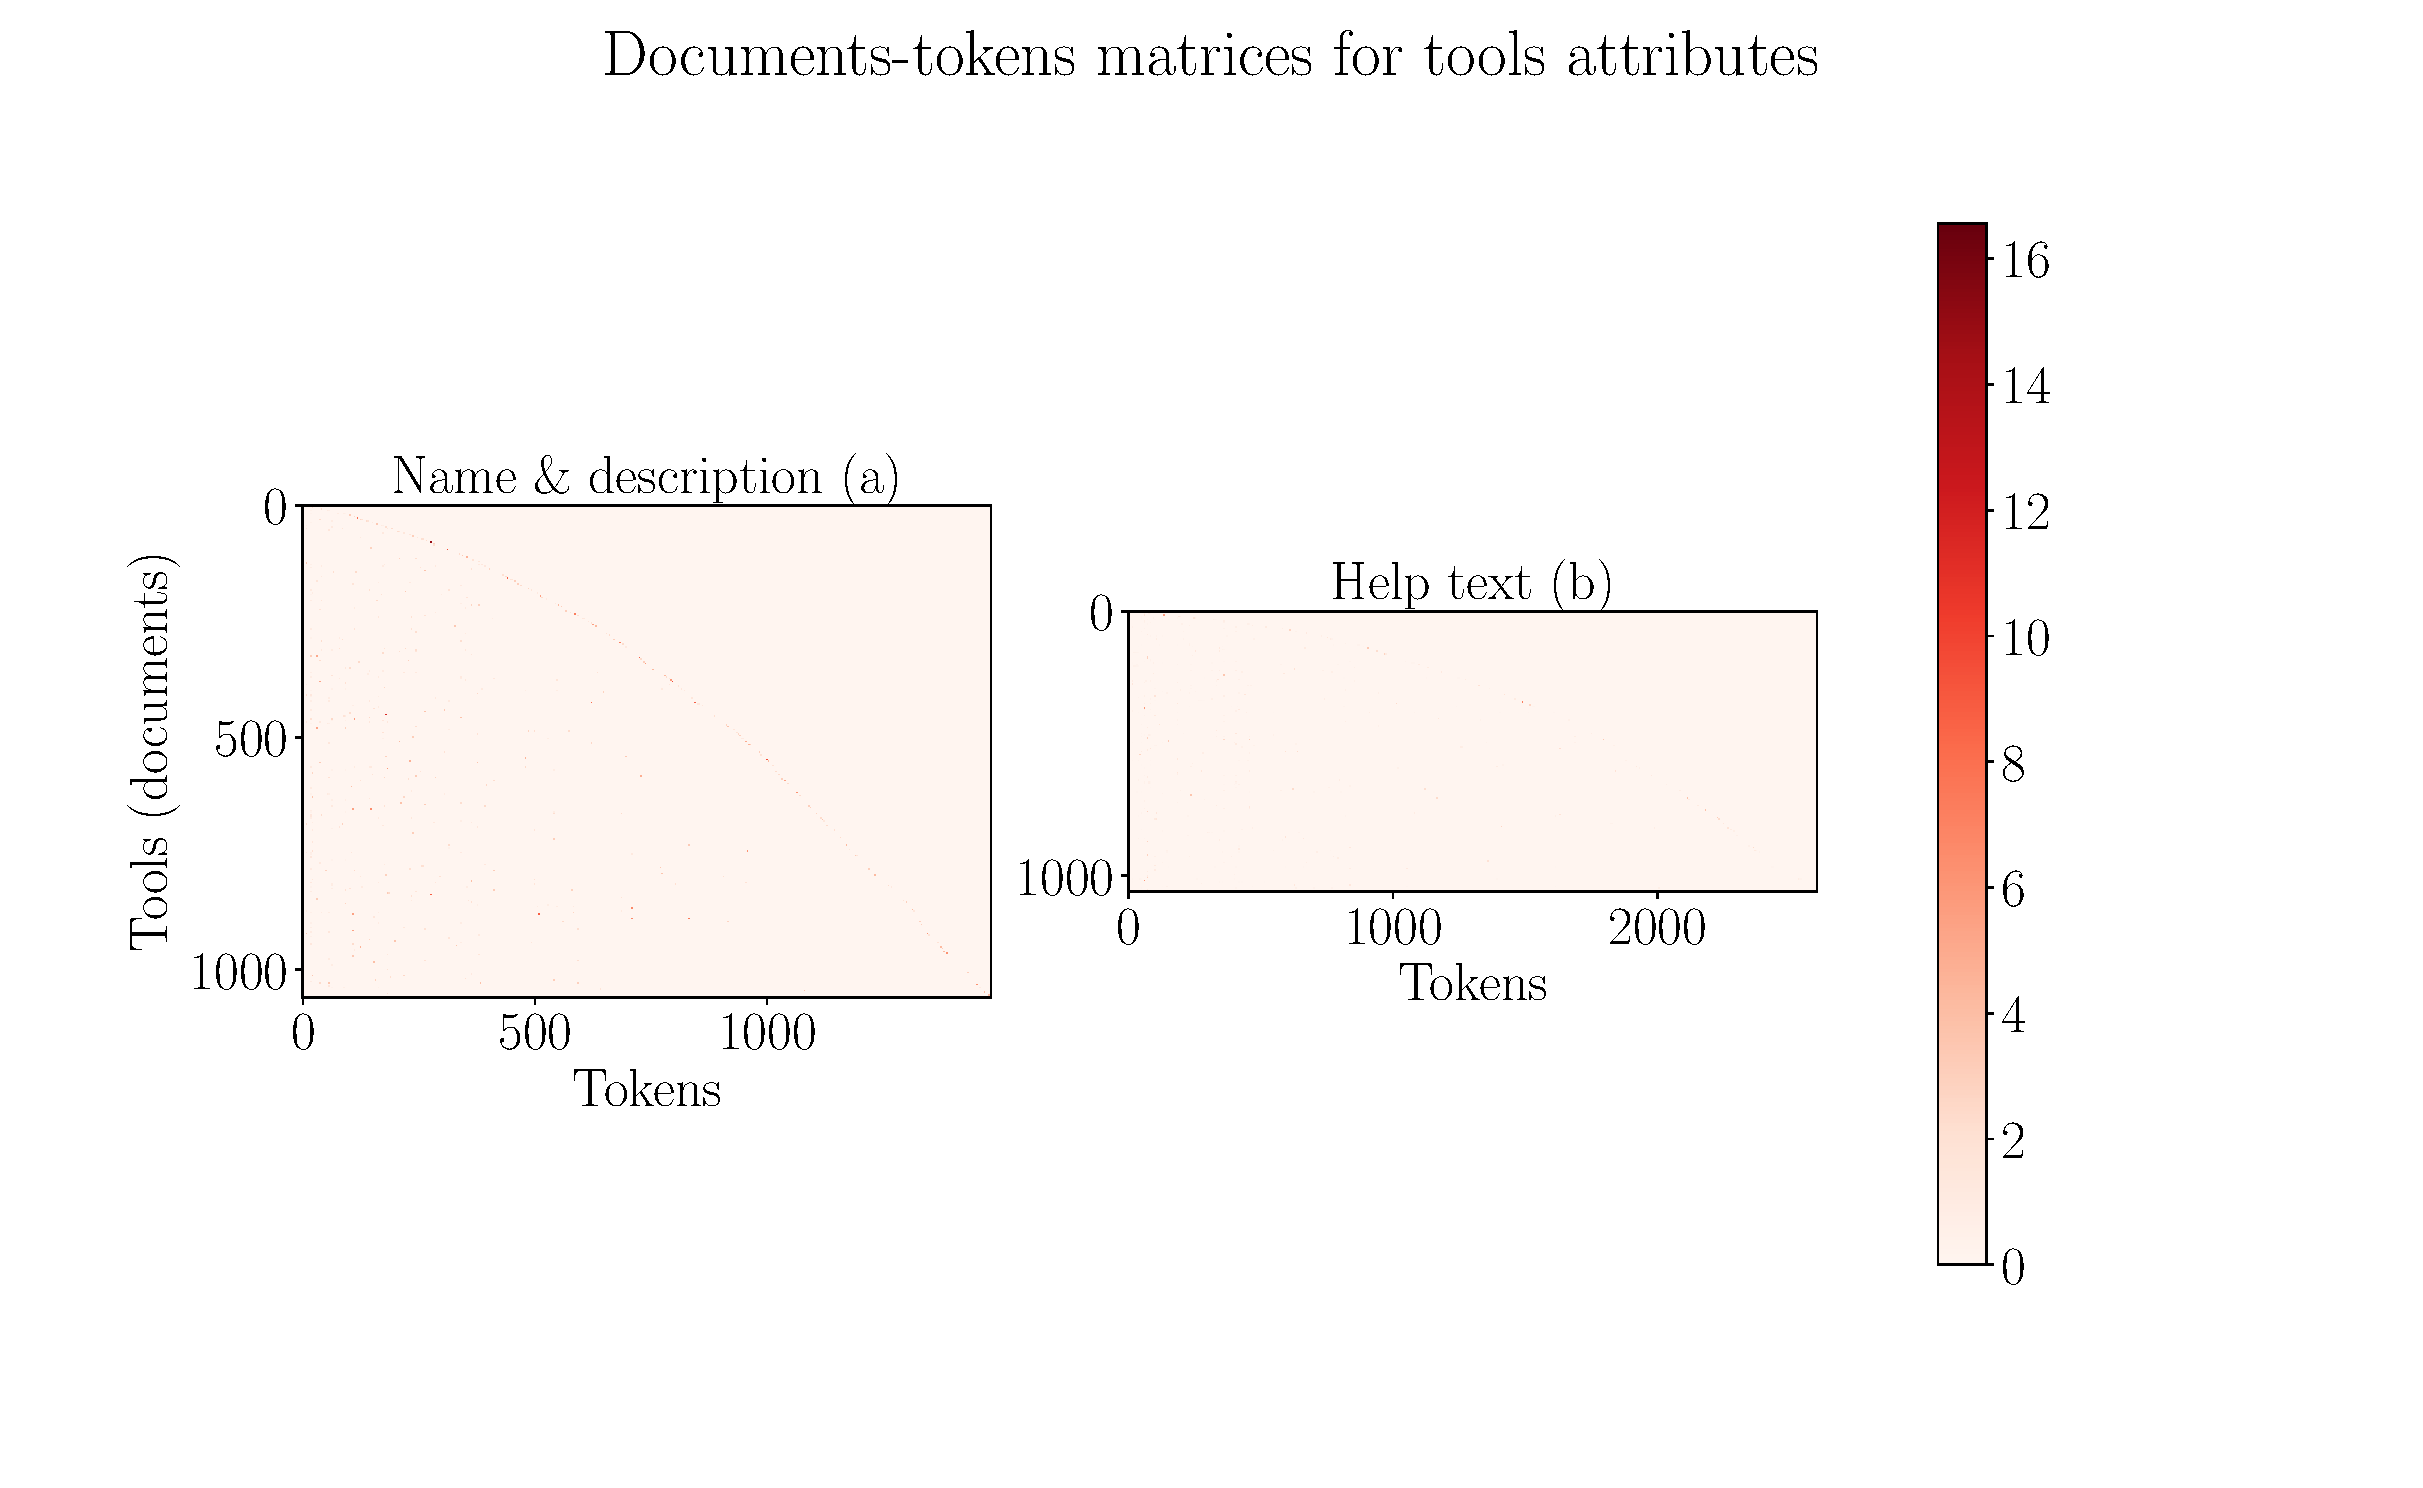
\includegraphics[scale=0.33]{figures/Document_tokens_full_rank.pdf}}
    \caption[Documents-tokens matrices]{\textbf{Documents-tokens matrices}: the heatmap shows the documents-tokens sparse matrices for two attributes.}
\end{centering}
\end{figure}

    
\section{Document embeddings}
\subsection{Latent semantic indexing}
    It is statistical way to learn the hidden concepts in documents by computing a low-rank representation of a documents-tokens matrix. This low-rank matrix is dense (figure 6). We use singular value decomposition ($SVD$) to decompose the full-rank matrix into a significantly lower rank matrix. The optimal rank to which a matrix to be decomposed is empirical in nature. The rank chosen still contains most of the singular values. This decomposition follows the equation:
    
    \begin{equation}
    X_{n \times m} = U_{n \times n} \cdot S_{n \times m} \cdot V_{m \times m}^T
    \end{equation}
    
    where $n$ is the number of documents and $m$ is the number of tokens. $S$ is a diagonal matrix containing the singular values in descending order. It contains the weights of the concepts present in the matrix. The matrices $U$ and $V$ and orthogonal matrices which satisfy:
    
    \begin{equation}
    U^T \cdot U = I_{n \times n}
    \end{equation}
    \begin{equation}
    V^T \cdot V = I_{m \times m}
    \end{equation}
    
\begin{figure}[h]
\begin{centering}
    {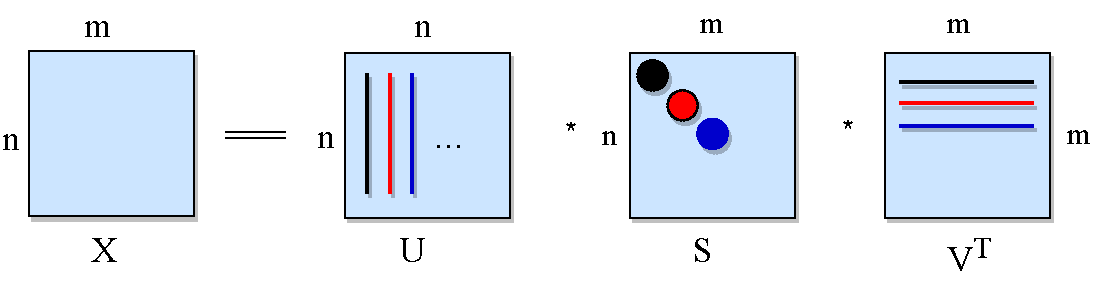
\includegraphics[scale=0.8]{figures/usv.pdf}}
    \caption[Pictorial representation of SVD]{\textbf{Pictorial representation of SVD}: the figure shows how singular value decomposition is done.}
\end{centering}
\end{figure}
    
    Figure 6 explains \footnote{\url{http://theory.stanford.edu/~tim/s15/l/l9.pdf}} 
    how $SVD$ of a matrix is carried out. The matrix $U$ contains information about how the tokens, arraged along the columns, are mapped to concepts and matrix $V$ stores information about how the concepts are mapped to documents arranged along the rows. 
    
    \subsubsection{Low-rank approximation}
    The low-rank approximation of a matrix is important to discard the features which are non-repeating or noise. Using this, we can collect the latent relations present in the documents-tokens matrices. We saw that our documents-tokens matrices suffer from sparseness and exhibit no relation among tokens. The approximation deals with these issues as well. The resulting matrices are dense and contain most of the singular values. The singular values which are small (the last entries of the $s$ matrix along the diagonal) are discarded \cite{DBLP:journals/corr/Yang15b}. The low-rank approximated matrix $X_k$ is computed as:
    \begin{equation}
    X_{nxm} = U_{k} \cdot S_{k} \cdot V_{k}^T
    \end{equation}
    where $U_{k}$ is the first $k$ columns of $U$, $V_{k}$ is the first $k$ rows and $S$ is the first $k$ singular values. $k$ is an empirical parameter. $X_k$ is called as the rank-k approximation of the full rank matrix $X$. Figure 7 shows the variation of the sum of singular values with the percentage rank of matrices. The percentage rank is $k \div K$ where $1 <= k <= K$ and $K$ is the original (full) rank of a matrix. We take it as the original ranks of the three matrices are not comparable. By doing this, we can show them on one plot. Similar idea we use for the sum of the singular values of each matrix. From figure 7, we can say that if we reduce the ranks of matrices to $70\%$ of the full-rank, we can still capture $\approx 90\%$ of the singular values. The reduction to half of the full-rank achieves $\approx 80\%$ of the sum of singular values. 

\begin{figure}[h]
\begin{centering}
    {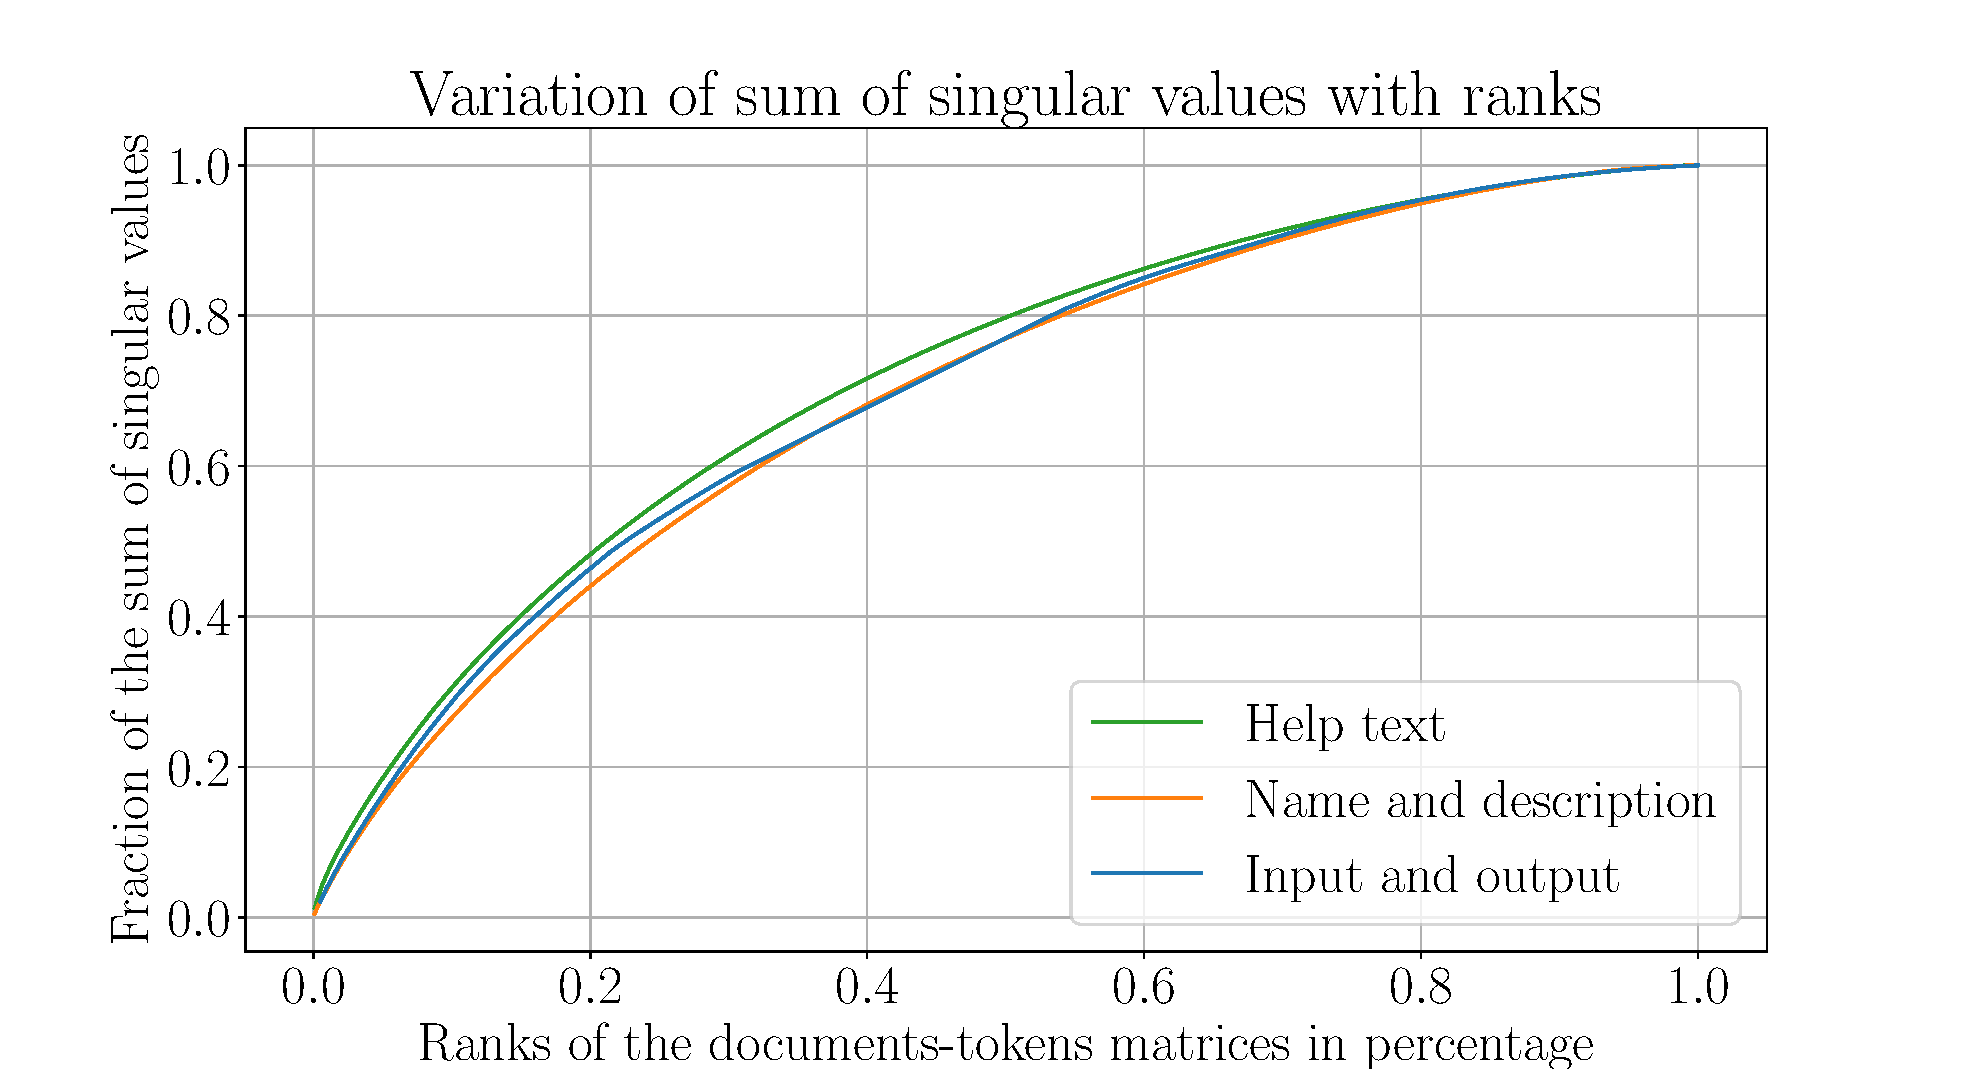
\includegraphics[scale=0.33]{figures/Rank_eigen_values.pdf}}
    \caption[Rank singular values]{\textbf{Matrix rank and singular values}: the plot shows how the sum of singular values vary with the rank of the documents-tokens matrix for all the attributes.}
\end{centering}
\end{figure}

We reduce the rank of the original documents-tokens matrices and compute the dense and approximated low-rank matrices. Figure 8 shows the low-rank matrices for input and output file types and name and description attributes. For computing this, we use only $40\%$ of the full-rank. We can compare it with figure 5 and deduce that figure 8 is denser than figure 5. In these low-rank matrices, we have dense vector representations for documents along the rows. In each matrix, each row contains a vector for one document. Using these documents vectors, we can compute the correlation or similarity using any similarity measure. There are multiple similarity measures that can be used like euclidean distance, cosine similarity, manhattan distance. We use cosine angle similarity to compute the correlation between vectors. By this, we get a positive real number between $0.0$ and $1.0$ specifying how similar a pair of documents are. The higher the score, higher is the similarity. Computing this similarity for all the documents give us a similarity matrix $S_{n \times n}$ where $n$ is the number of documents. This square, symmetric matrix is called as similarity or correlation matrix. We compute three such matrices each corresponding to one attribute.
  
\begin{figure}[h]
\begin{centering}
    {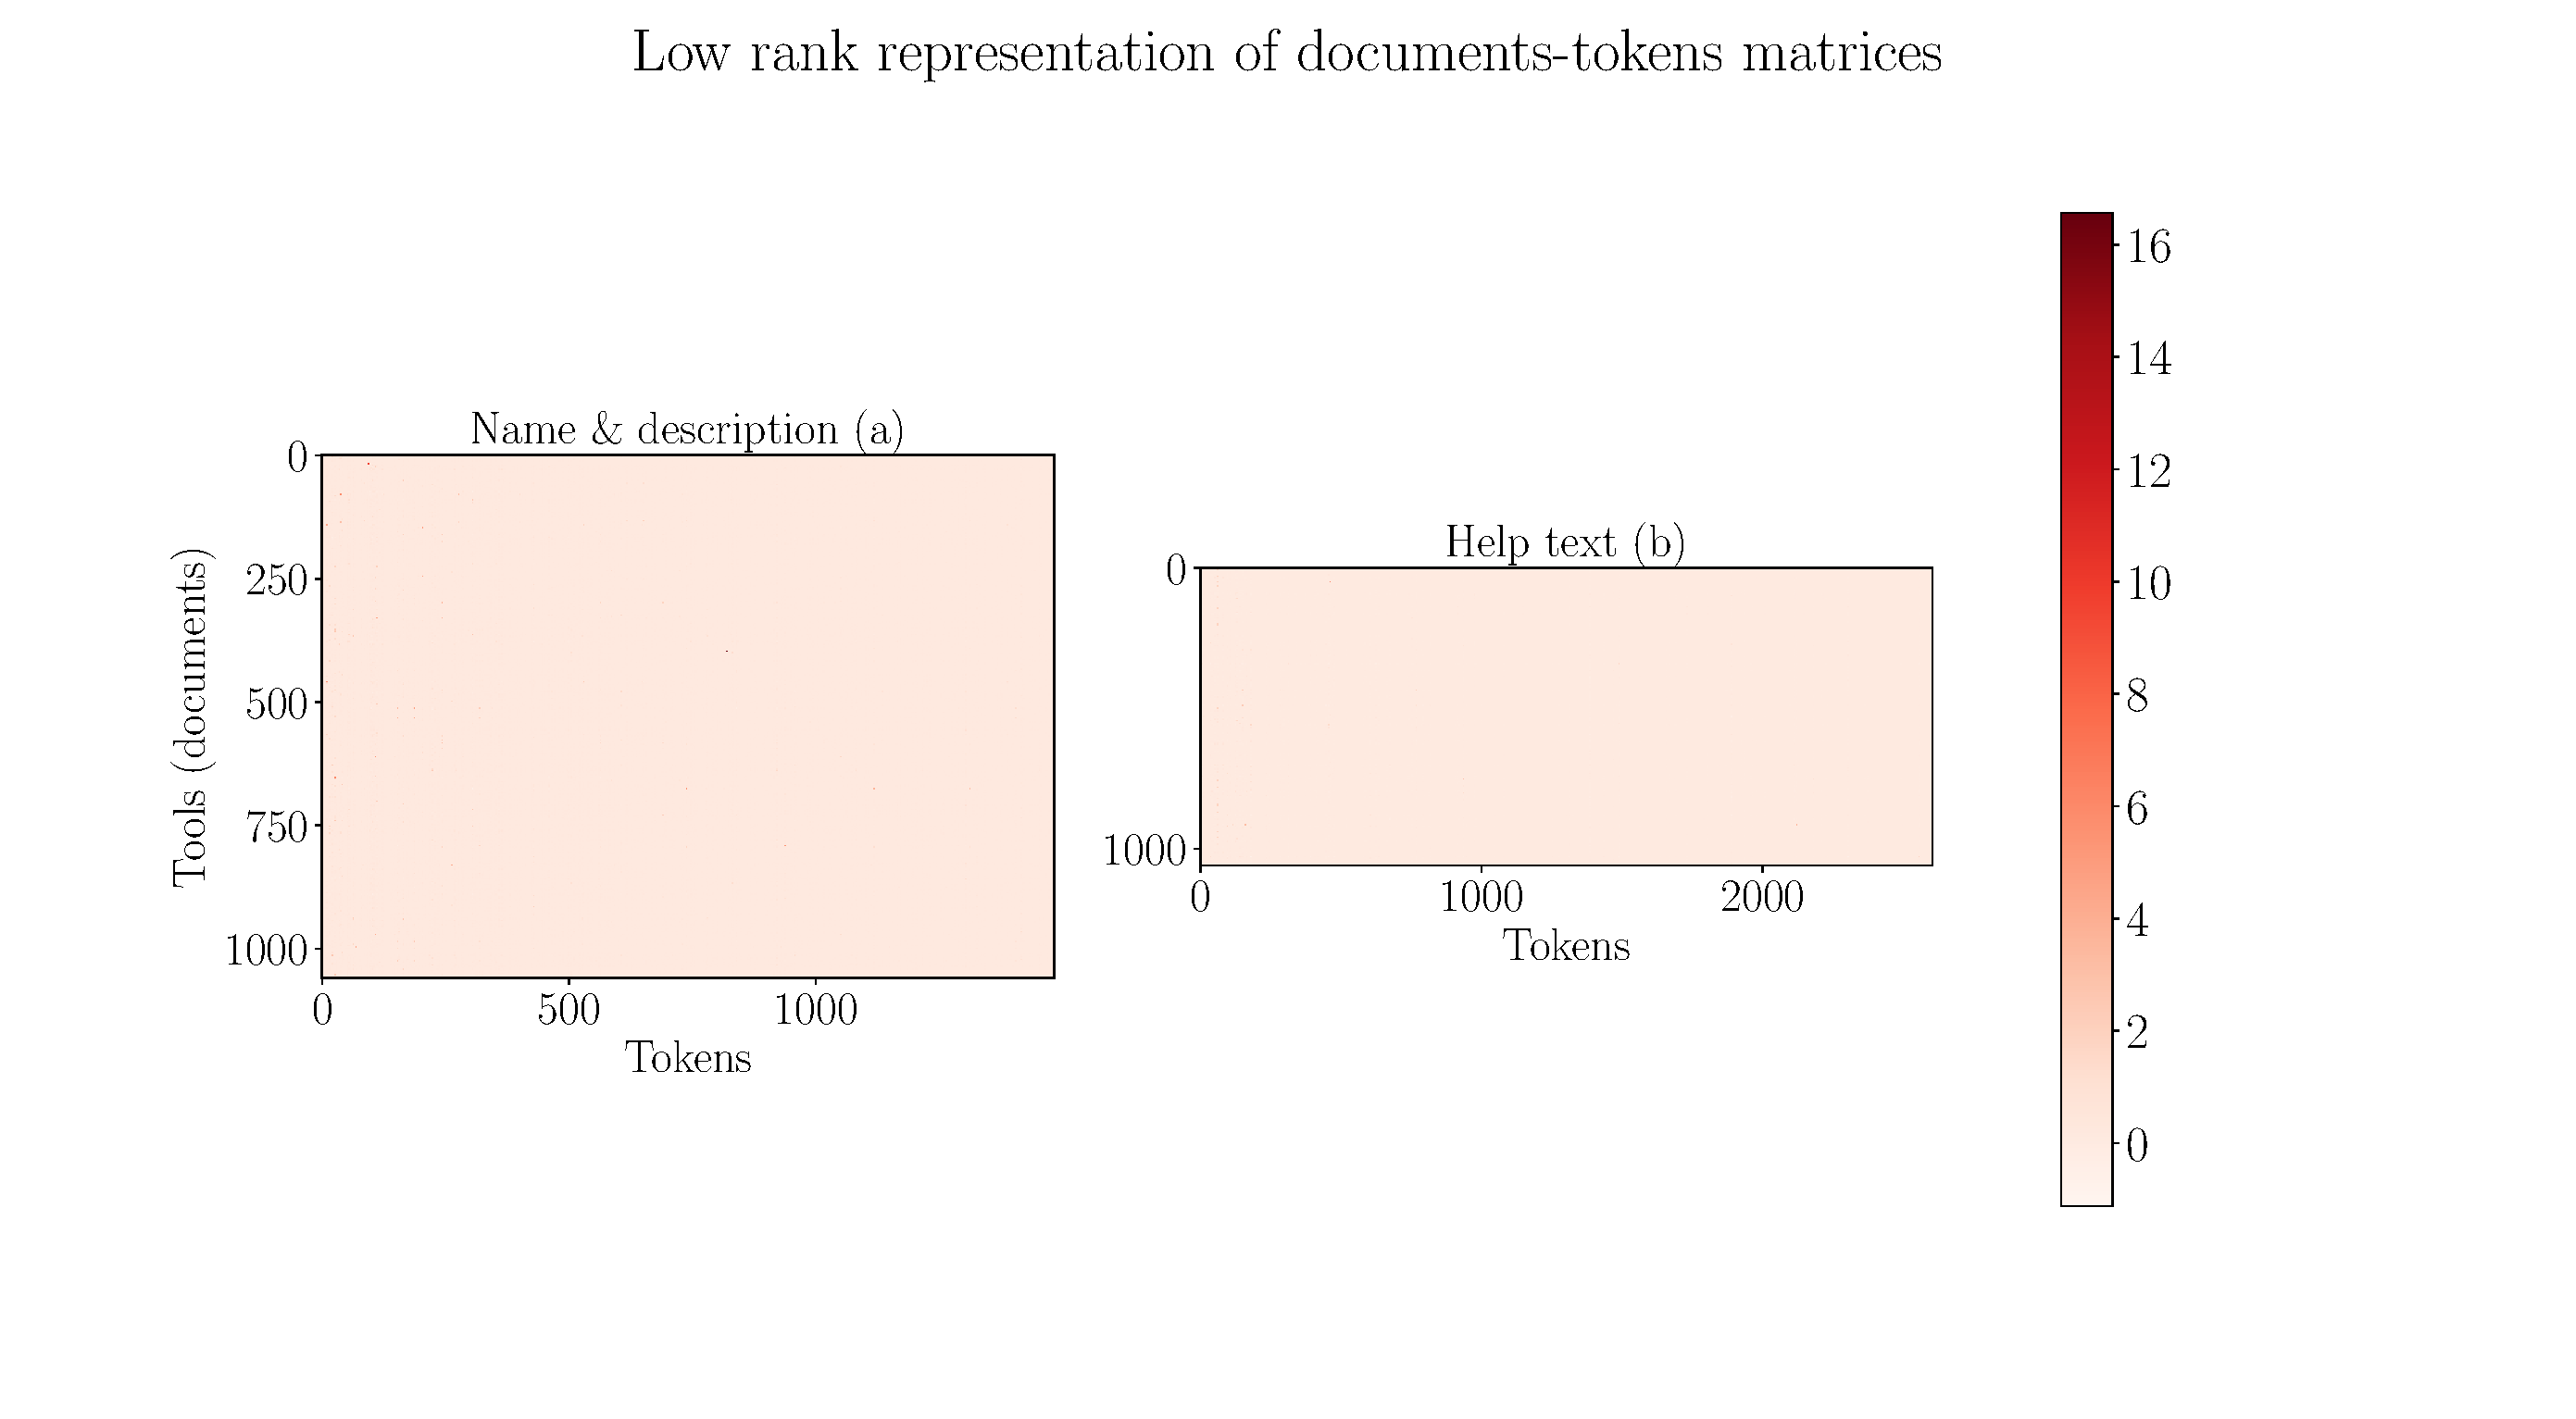
\includegraphics[scale=0.33]{figures/Document_tokens_low_rank.pdf}}
    \caption[Documents-tokens matrices]{\textbf{Documents-tokens matrices}: the heatmap shows the documents-tokens low rank representation of the matrices.}
\end{centering}
\end{figure}

\subsection{Paragraph vectors}


\section{Similarity measures}
    \subsubsection{Cosine similarity}

\section{Optimization}
\subsubsection{Gradient descent}
\subsubsection{Backtracking line search}